\documentclass[12pt,letterpaper]{article}
\usepackage{graphicx,textcomp}
\usepackage{natbib}
\usepackage{setspace}
\usepackage{fullpage}
\usepackage{color}
\usepackage[reqno]{amsmath}
\usepackage{amsthm}
\usepackage{fancyvrb}
\usepackage{amssymb,enumerate}
\usepackage[all]{xy}
\usepackage{endnotes}
\usepackage{lscape}
\newtheorem{com}{Comment}
\usepackage{float}
\usepackage{hyperref}
\newtheorem{lem} {Lemma}
\newtheorem{prop}{Proposition}
\newtheorem{thm}{Theorem}
\newtheorem{defn}{Definition}
\newtheorem{cor}{Corollary}
\newtheorem{obs}{Observation}
\usepackage[compact]{titlesec}
\usepackage{dcolumn}
\usepackage{tikz}
\usetikzlibrary{arrows}
\usepackage{multirow}
\usepackage{xcolor}
\newcolumntype{.}{D{.}{.}{-1}}
\newcolumntype{d}[1]{D{.}{.}{#1}}
\definecolor{light-gray}{gray}{0.65}
\usepackage{url}
\usepackage{listings}
\usepackage{color}

\definecolor{codegreen}{rgb}{0,0.6,0}
\definecolor{codegray}{rgb}{0.5,0.5,0.5}
\definecolor{codepurple}{rgb}{0.58,0,0.82}
\definecolor{backcolour}{rgb}{0.95,0.95,0.92}

\lstdefinestyle{mystyle}{
	backgroundcolor=\color{backcolour},   
	commentstyle=\color{codegreen},
	keywordstyle=\color{magenta},
	numberstyle=\tiny\color{codegray},
	stringstyle=\color{codepurple},
	basicstyle=\footnotesize,
	breakatwhitespace=false,         
	breaklines=true,                 
	captionpos=b,                    
	keepspaces=true,                 
	numbers=left,                    
	numbersep=5pt,                  
	showspaces=false,                
	showstringspaces=false,
	showtabs=false,                  
	tabsize=2
}
\lstset{style=mystyle}
\newcommand{\Sref}[1]{Section~\ref{#1}}
\newtheorem{hyp}{Hypothesis}

\title{Problem Set 3}
\date{Due: November 19, 2022}
\author{Applied Stats/Quant Methods 1}


\begin{document}
	\maketitle
	\section*{Instructions}
	\begin{itemize}
		\item Please show your work! You may lose points by simply writing in the answer. If the problem requires you to execute commands in \texttt{R}, please include the code you used to get your answers. Please also include the \texttt{.R} file that contains your code. If you are not sure if work needs to be shown for a particular problem, please ask.
	\item Your homework should be submitted electronically on GitHub.
	\item This problem set is due before 23:59 on Sunday November 19, 2023. No late assignments will be accepted.

	\end{itemize}

		\vspace{.25cm}
	
\noindent In this problem set, you will run several regressions and create an add variable plot (see the lecture slides) in \texttt{R} using the \texttt{incumbents\_subset.csv} dataset. Include all of your code.

	\vspace{.5cm}
\section*{Question 1}
\vspace{.25cm}
\noindent We are interested in knowing how the difference in campaign spending between incumbent and challenger affects the incumbent's vote share. 
	\begin{enumerate}
		\item Run a regression where the outcome variable is \texttt{voteshare} and the explanatory variable is \texttt{difflog}.
		
\textbf{		The R script for regression is:}
		\lstinputlisting[language=R, firstline=41, lastline=42]{PS3.R}  
		
		The intercept is 0.579 while the slope of this regression line is 0.041. The R squared value of 0.37 means that around 37 percent of the variability in the voteshare (response variable) can be explained by difflog (explanatory variable). The p-value shows that the difference in campaign spending between incumbent and challenger is a significant predictor of incumbents' vote share.
		
		
		\item Make a scatterplot of the two variables and add the regression line. 
		
		\lstinputlisting[language=R, firstline=45, lastline=48]{PS3.R}  
		
		
		\begin{figure}[h!]\centering	\caption{\footnotesize Scatterplot of relationship between $voteshare, difflog$.}	
		
		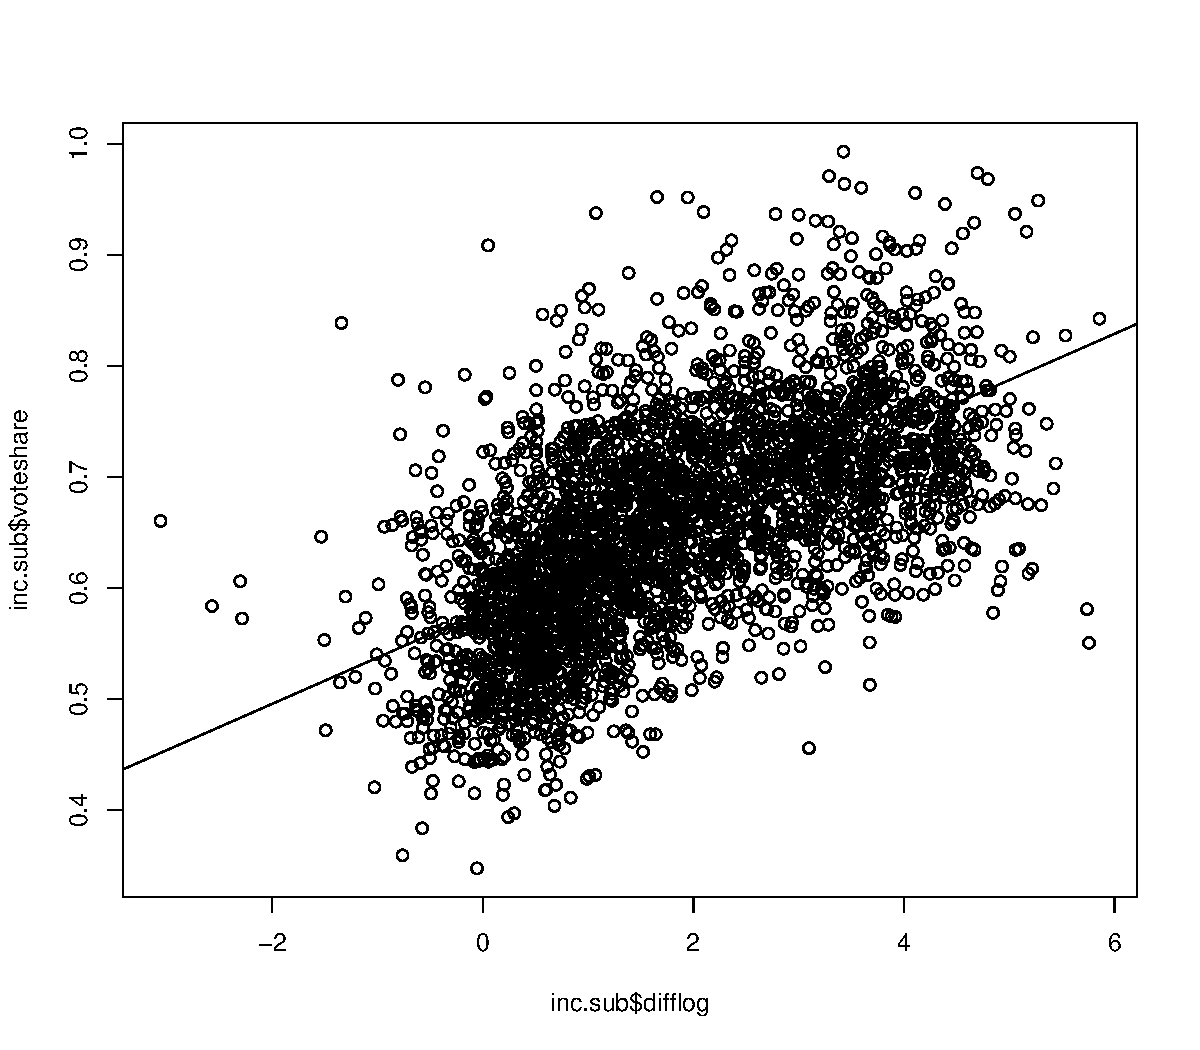
\includegraphics[width=.85\textwidth]{plot1.pdf}
		
		\end{figure}
		
		The above scatter plot shows a positive linear relationship between the variables.    
		
		\vspace*{2cm}
		
		\item Save the residuals of the model in a separate object.			
		\lstinputlisting[language=R, firstline=51, lastline=51]{PS3.R}
		
		The negative residual value shows that the model overestimates the incumbents' vote share and it is less than predicted by the model. 
		
		\item Write the prediction equation.
		
		voteshare = \textit{B0} +\textit{B1} * difflog
		
		The intercept is 0.579 while the slope of this regression line is 0.041 which means that with every percentage point increase in the difference of campaign spending between incumbent and challenger, we would expect the percentage increase in voteshare to be increased by 0.041 percent points.
		 
	\end{enumerate}
	
\newpage

\section*{Question 2}
\noindent We are interested in knowing how the difference between incumbent and challenger's spending and the vote share of the presidential candidate of the incumbent's party are related.	\vspace{.25cm}
	\begin{enumerate}
		\item Run a regression where the outcome variable is \texttt{presvote} and the explanatory variable is \texttt{difflog}.
		
		
		
		\textbf{		The R script for regression is:}
		\lstinputlisting[language=R, firstline=58, lastline=59]{PS3.R}  
		
		
		The intercept is 0.507 while the slope of this regression line is 0.024. The R squared value of 0.087 means that around 9 percent of the variability in the presvote (response variable) can be explained by difflog (explanatory variable). The p-value shows that the difference in campaign spending between incumbent and challenger is a significant predictor of presvote.
		
		\item Make a scatterplot of the two variables and add the regression line. 
		
			\lstinputlisting[language=R, firstline=62, lastline=65]{PS3.R}  
		
		
		\begin{figure}[h!]\centering	\caption{\footnotesize Scatterplot of relationship between $Y, X_2$.}	
			
			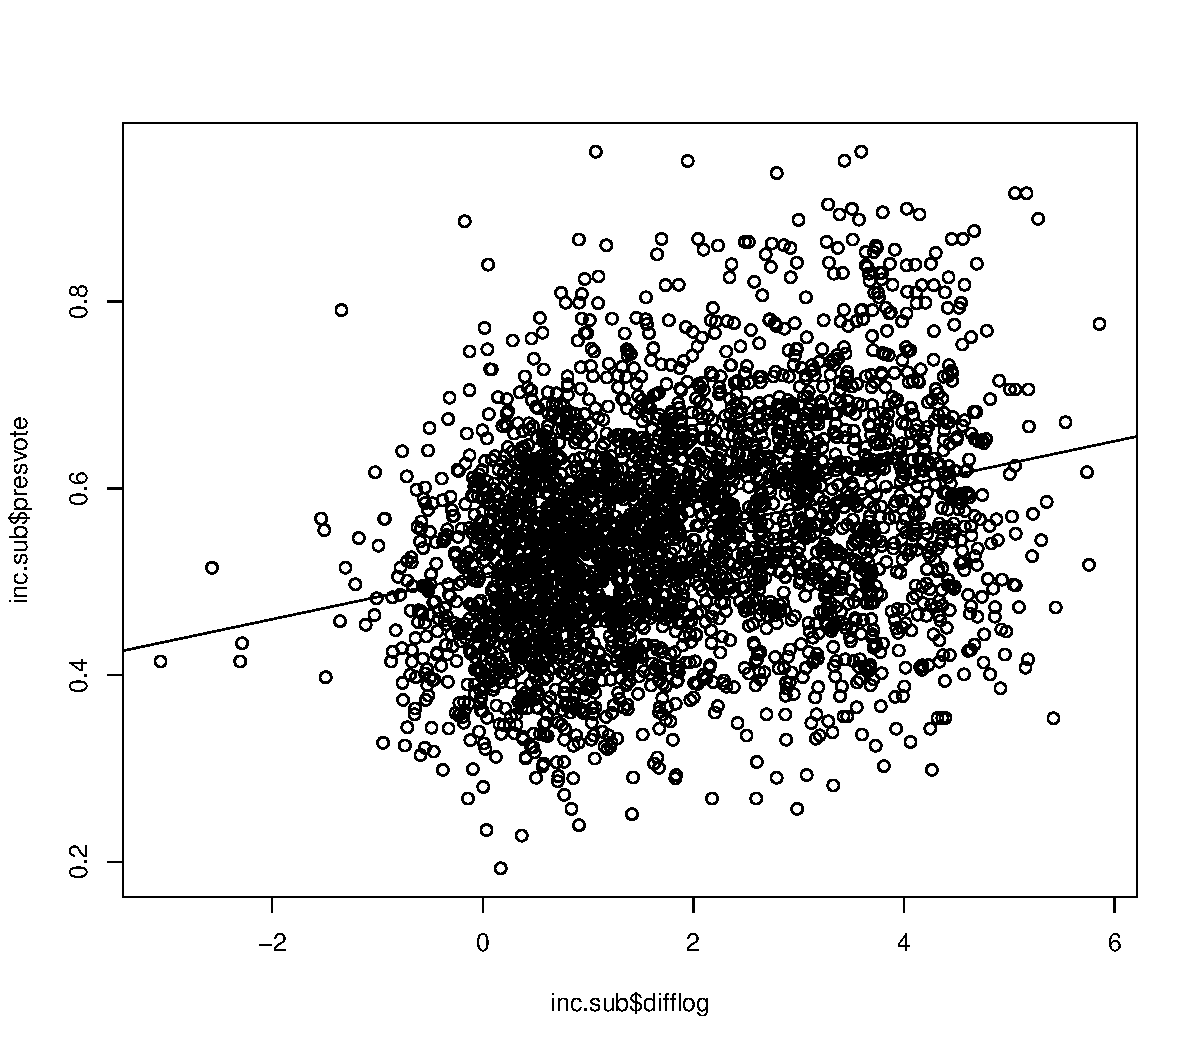
\includegraphics[width=.6\textwidth]{plot2.pdf}
			
		\end{figure}
		
		The above scatter plot shows a positive linear relationship between the variables.
		
		\newpage	
		\item Save the residuals of the model in a separate object.
		
		\lstinputlisting[language=R, firstline=70, lastline=70]{PS3.R}
		
		The positive residual value shows that the model underestimates the presvote  and it is more than predicted by the model. 
		
		
		\item Write the prediction equation.
		
		
		presvote = \textit{B0} +\textit{B1} * difflog
		
		The intercept is 0.507 while the slope of this regression line is 0.024 which means that with every percentage point increase in the difference of campaign spending between incumbent and challenger, we would expect the percentage increase in presvote to be increased by 0.024 percent points.
		
	\end{enumerate}
	
	\newpage	
	
\section*{Question 3}

\noindent We are interested in knowing how the vote share of the presidential candidate of the incumbent's party is associated with the incumbent's electoral success.
	\vspace{.25cm}
	\begin{enumerate}
		\item Run a regression where the outcome variable is \texttt{voteshare} and the explanatory variable is \texttt{presvote}.
			\textbf{		The R script for regression is:}
		\lstinputlisting[language=R, firstline=76, lastline=77]{PS3.R}  
		
		The intercept is 0.441 while the slope of this regression line is 0.388. The R squared value of 0.20 means that around 20 percent of the variability in the voteshare (response variable) can be explained by presvote (explanatory variable). The p-value shows that the difference in campaign spending between incumbent and challenger is a significant predictor of incumbents' vote share.
			
			
		\item Make a scatterplot of the two variables and add the regression line. 
			
			
			\lstinputlisting[language=R, firstline=80, lastline=83]{PS3.R} 
				\begin{figure}[h!]\centering	\caption{\footnotesize Scatterplot of relationship between $voteshare, presvote$.}	
				
				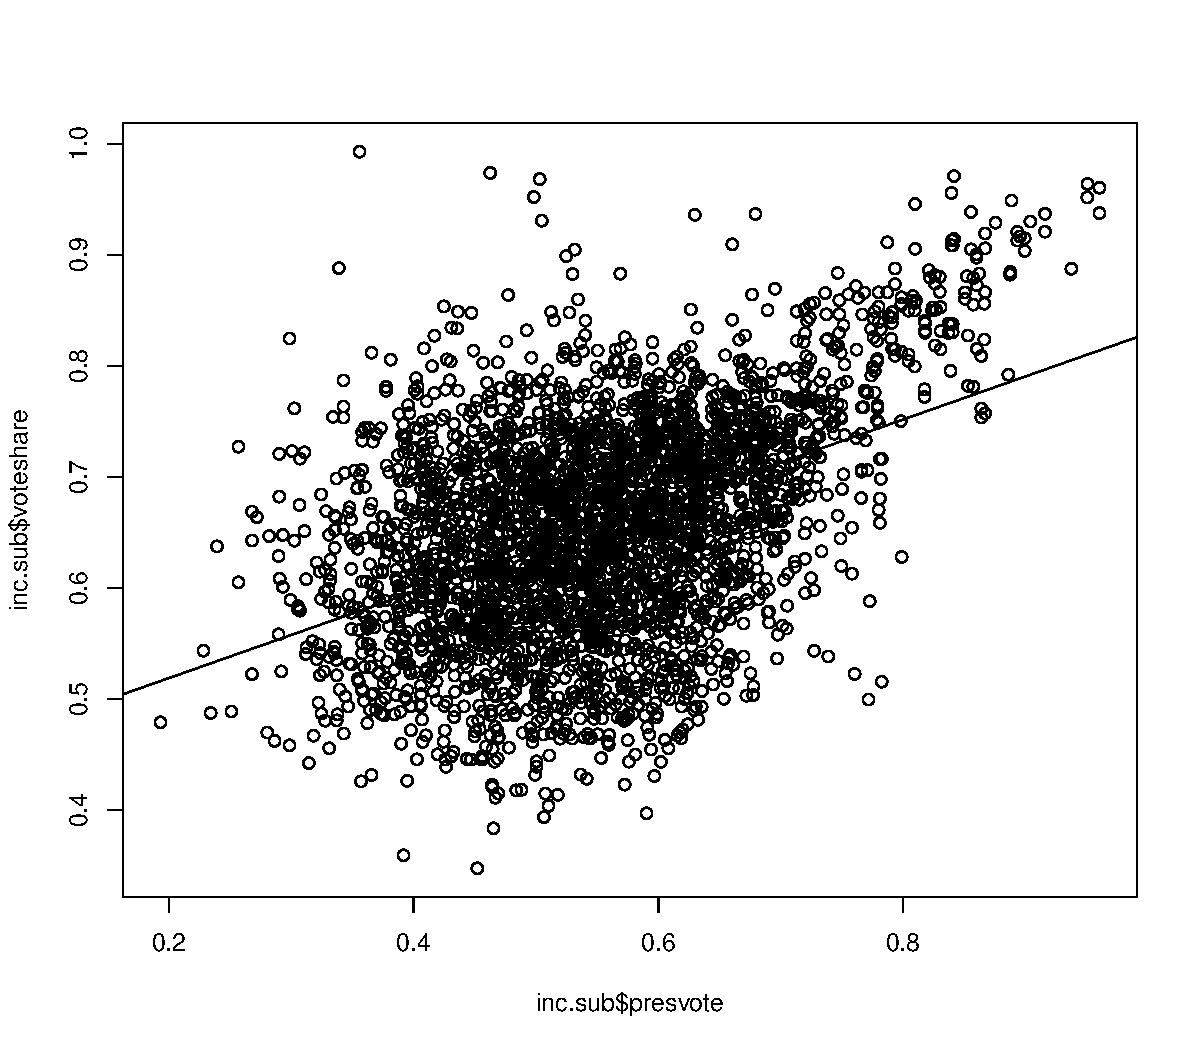
\includegraphics[width=.65\textwidth]{plot3.pdf}
				
			\end{figure}
			
			
			The above scatter plot shows a positive linear relationship between the variables.
			
			
		\item Write the prediction equation.
		
		voteshare = \textit{B0} + \textit{B1} * presvote
		
		The intercept is 0.441 while the slope of this regression line is 0.388 which means that with every percentage point increase in the presvote, we would expect the percentage increase in voteshare to be increased by 0.388 percent points.
		
		
		
		
	\end{enumerate}
	

\newpage	

\section*{Question 4}
\noindent The residuals from part (a) tell us how much of the variation in \texttt{voteshare} is $not$ explained by the difference in spending between incumbent and challenger. The residuals in part (b) tell us how much of the variation in \texttt{presvote} is $not$ explained by the difference in spending between incumbent and challenger in the district.
	\begin{enumerate}
		\item Run a regression where the outcome variable is the residuals from Question 1 and the explanatory variable is the residuals from Question 2.
		
		\textbf{		The R script for regression is:}
		\lstinputlisting[language=R, firstline=91, lastline=92]{PS3.R} 
		
		
		Both the intercept and slope are having very smaller values. The multiple R squared value of 0.13 means that around 13 percent of the variability in the 1st residual (response variable) can be explained by 2nd residual (explanatory variable). The p-value shows that residual 2 is a significant predictor of residual 1.
		
		\item Make a scatterplot of the two residuals and add the regression line. 
		
		
		\lstinputlisting[language=R, firstline=95, lastline=98]{PS3.R}  
		
		
		\begin{figure}[h!]\centering	\caption{\footnotesize Scatterplot of relationship between $res1, res2$.}	
			
			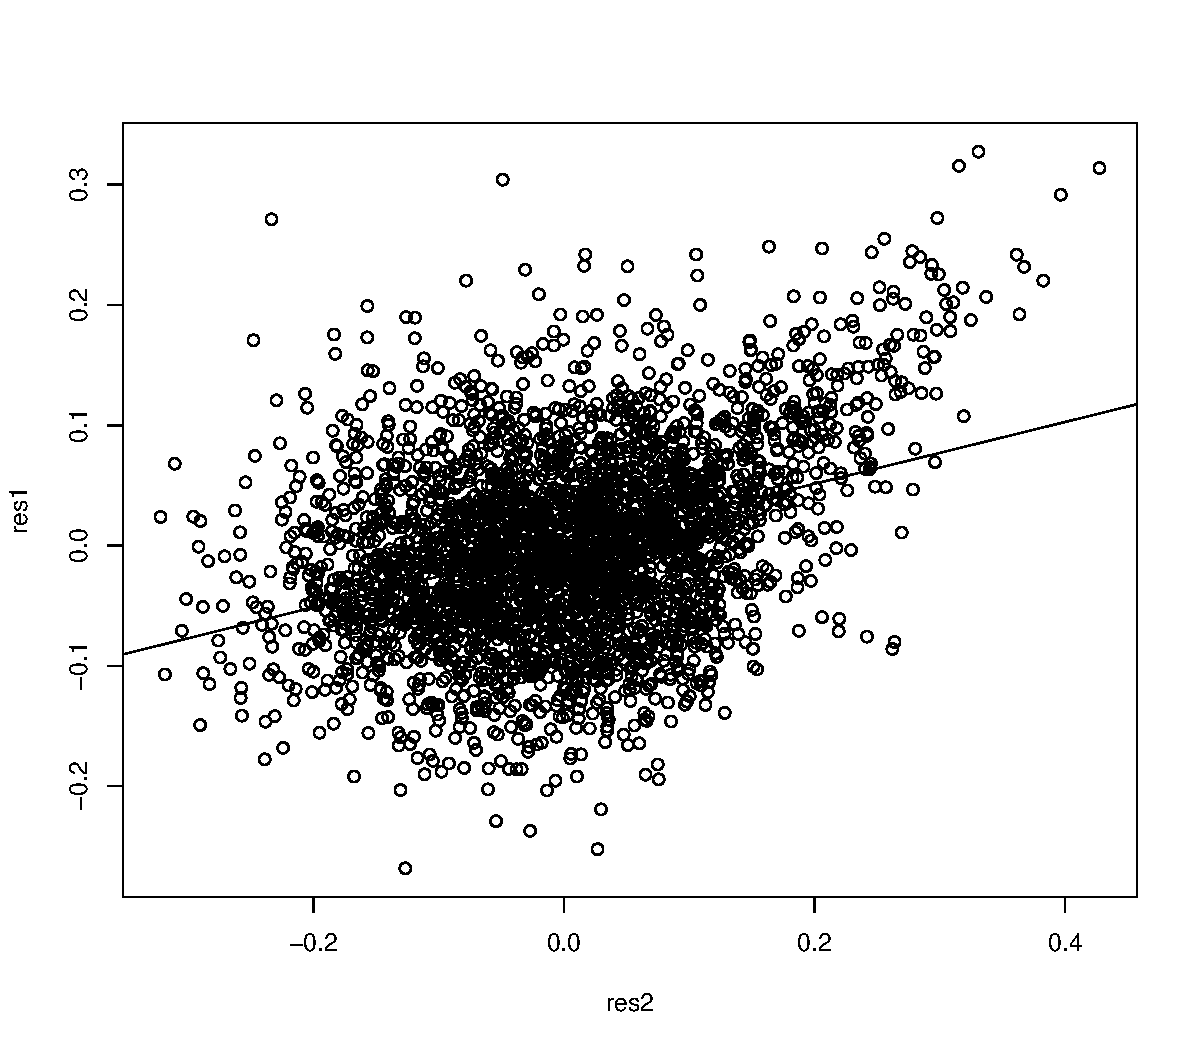
\includegraphics[width=.6\textwidth]{plot4.pdf}
			
		\end{figure}
		
		The above scatter plot shows a positive linear relationship between the variables.
		
		
		\item Write the prediction equation.
	
	
	res1 = \textit{B0} + \textit{B1} * res2
	
	
	The intercept and slope of this regression line is very smaller which means that with every percentage point increase in the residual2, we would expect a tiny percentage increase in residual1.
	
	\end{enumerate}
	
	\newpage	

\section*{Question 5}
\noindent What if the incumbent's vote share is affected by both the president's popularity and the difference in spending between incumbent and challenger? 
	\begin{enumerate}
		\item Run a regression where the outcome variable is the incumbent's \texttt{voteshare} and the explanatory variables are \texttt{difflog} and \texttt{presvote}.
	
	
		\textbf{		The R script for regression is:}
		\lstinputlisting[language=R, firstline=104, lastline=105]{PS3.R} 
	
	
		The intercept is 0.448 while the slopes are 0.0355 and 0.256 respectively. The R squared value of 0.45 means that around 45 percent of the variability in the voteshare (response variable) can be explained by presvote and difference in campaign spending between incumbents and challenger (explanatory variables). The p-value shows that the difference in campaign spending between incumbent and challenger and presvote are significant predictors of incumbents' vote share.
	
		\item Write the prediction equation.
	
	
		voteshare = \textit{B0} + \textit{B1} * difflog + \textit{B2} * presvote
	
		The intercept is 0.448 while the slope of 0.0355 and 0.256 means that with every percentage point increase in the difference in campaign spending between the incumbent and challenger, we would expect the percentage increase in voteshare to be increased by 0.0355 percent points while with every percentage point increase in the presvote, we would expect the percentage increase in voteshare to be increased by 0.256 percentage points.
	
	
		\item What is it in this output that is identical to the output in Question 4? Why do you think this is the case?
	
		In both Question 4 and Question 5, although the p-value indicates that there is a significant relationship between the explanatory and response variables\\
		, the R squared value and multiple R squared values are low which indicates that there are other variables that may have a significant impact on the incumbents' vote share.   
	
	\end{enumerate}




\end{document}
